% Options for packages loaded elsewhere
% Options for packages loaded elsewhere
\PassOptionsToPackage{unicode}{hyperref}
\PassOptionsToPackage{hyphens}{url}
\PassOptionsToPackage{dvipsnames,svgnames,x11names}{xcolor}
%
\documentclass[
  11pt,
  a4paper,
]{article}
\usepackage{xcolor}
\usepackage[margin=1in]{geometry}
\usepackage{amsmath,amssymb}
\setcounter{secnumdepth}{-\maxdimen} % remove section numbering
\usepackage{iftex}
\ifPDFTeX
  \usepackage[T1]{fontenc}
  \usepackage[utf8]{inputenc}
  \usepackage{textcomp} % provide euro and other symbols
\else % if luatex or xetex
  \usepackage{unicode-math} % this also loads fontspec
  \defaultfontfeatures{Scale=MatchLowercase}
  \defaultfontfeatures[\rmfamily]{Ligatures=TeX,Scale=1}
\fi
\usepackage{lmodern}
\ifPDFTeX\else
  % xetex/luatex font selection
\fi
% Use upquote if available, for straight quotes in verbatim environments
\IfFileExists{upquote.sty}{\usepackage{upquote}}{}
\IfFileExists{microtype.sty}{% use microtype if available
  \usepackage[]{microtype}
  \UseMicrotypeSet[protrusion]{basicmath} % disable protrusion for tt fonts
}{}
\makeatletter
\@ifundefined{KOMAClassName}{% if non-KOMA class
  \IfFileExists{parskip.sty}{%
    \usepackage{parskip}
  }{% else
    \setlength{\parindent}{0pt}
    \setlength{\parskip}{6pt plus 2pt minus 1pt}}
}{% if KOMA class
  \KOMAoptions{parskip=half}}
\makeatother
% Make \paragraph and \subparagraph free-standing
\makeatletter
\ifx\paragraph\undefined\else
  \let\oldparagraph\paragraph
  \renewcommand{\paragraph}{
    \@ifstar
      \xxxParagraphStar
      \xxxParagraphNoStar
  }
  \newcommand{\xxxParagraphStar}[1]{\oldparagraph*{#1}\mbox{}}
  \newcommand{\xxxParagraphNoStar}[1]{\oldparagraph{#1}\mbox{}}
\fi
\ifx\subparagraph\undefined\else
  \let\oldsubparagraph\subparagraph
  \renewcommand{\subparagraph}{
    \@ifstar
      \xxxSubParagraphStar
      \xxxSubParagraphNoStar
  }
  \newcommand{\xxxSubParagraphStar}[1]{\oldsubparagraph*{#1}\mbox{}}
  \newcommand{\xxxSubParagraphNoStar}[1]{\oldsubparagraph{#1}\mbox{}}
\fi
\makeatother


\usepackage{longtable,booktabs,array}
\usepackage{calc} % for calculating minipage widths
% Correct order of tables after \paragraph or \subparagraph
\usepackage{etoolbox}
\makeatletter
\patchcmd\longtable{\par}{\if@noskipsec\mbox{}\fi\par}{}{}
\makeatother
% Allow footnotes in longtable head/foot
\IfFileExists{footnotehyper.sty}{\usepackage{footnotehyper}}{\usepackage{footnote}}
\makesavenoteenv{longtable}
\usepackage{graphicx}
\makeatletter
\newsavebox\pandoc@box
\newcommand*\pandocbounded[1]{% scales image to fit in text height/width
  \sbox\pandoc@box{#1}%
  \Gscale@div\@tempa{\textheight}{\dimexpr\ht\pandoc@box+\dp\pandoc@box\relax}%
  \Gscale@div\@tempb{\linewidth}{\wd\pandoc@box}%
  \ifdim\@tempb\p@<\@tempa\p@\let\@tempa\@tempb\fi% select the smaller of both
  \ifdim\@tempa\p@<\p@\scalebox{\@tempa}{\usebox\pandoc@box}%
  \else\usebox{\pandoc@box}%
  \fi%
}
% Set default figure placement to htbp
\def\fps@figure{htbp}
\makeatother





\setlength{\emergencystretch}{3em} % prevent overfull lines

\providecommand{\tightlist}{%
  \setlength{\itemsep}{0pt}\setlength{\parskip}{0pt}}






\usepackage{amsmath,amssymb,amsthm}
\usepackage{mathtools}
\usepackage{unicode-math}
\makeatletter
\@ifpackageloaded{caption}{}{\usepackage{caption}}
\AtBeginDocument{%
\ifdefined\contentsname
  \renewcommand*\contentsname{Table of contents}
\else
  \newcommand\contentsname{Table of contents}
\fi
\ifdefined\listfigurename
  \renewcommand*\listfigurename{List of Figures}
\else
  \newcommand\listfigurename{List of Figures}
\fi
\ifdefined\listtablename
  \renewcommand*\listtablename{List of Tables}
\else
  \newcommand\listtablename{List of Tables}
\fi
\ifdefined\figurename
  \renewcommand*\figurename{Figure}
\else
  \newcommand\figurename{Figure}
\fi
\ifdefined\tablename
  \renewcommand*\tablename{Table}
\else
  \newcommand\tablename{Table}
\fi
}
\@ifpackageloaded{float}{}{\usepackage{float}}
\floatstyle{ruled}
\@ifundefined{c@chapter}{\newfloat{codelisting}{h}{lop}}{\newfloat{codelisting}{h}{lop}[chapter]}
\floatname{codelisting}{Listing}
\newcommand*\listoflistings{\listof{codelisting}{List of Listings}}
\makeatother
\makeatletter
\makeatother
\makeatletter
\@ifpackageloaded{caption}{}{\usepackage{caption}}
\@ifpackageloaded{subcaption}{}{\usepackage{subcaption}}
\makeatother
\usepackage{bookmark}
\IfFileExists{xurl.sty}{\usepackage{xurl}}{} % add URL line breaks if available
\urlstyle{same}
\hypersetup{
  pdftitle={Definition: Image},
  colorlinks=true,
  linkcolor={blue},
  filecolor={Maroon},
  citecolor={Blue},
  urlcolor={Blue},
  pdfcreator={LaTeX via pandoc}}


\title{Definition: Image}
\author{}
\date{}
\begin{document}
\maketitle


\section{Definition: Image}\label{def-image}

Let \(T: V \to W\) be a \href{def-linear-transformation.qmd}{Linear
Transformation} between \href{def-vector-space.qmd}{s}. The
\textbf{image} (or \textbf{range}) of \(T\) is the set of all vectors in
\(W\) that are outputs of \(T\):

\[\text{im}(T) = \{T(\mathbf{v}) : \mathbf{v} \in V\} = T(V)\]

\subsection{Alternative Names}\label{alternative-names}

The image is also known as: - Range (denoted \(\text{range}(T)\) or
\(R(T)\)) - The image of the domain under \(T\)

\subsection{Properties}\label{properties}

\begin{enumerate}
\def\labelenumi{\arabic{enumi}.}
\item
  \textbf{Subspace}: \(\text{im}(T)\) is always a subspace of \(W\)

  \begin{itemize}
  \tightlist
  \item
    Contains \(\mathbf{0}_W\) since \(T(\mathbf{0}_V) = \mathbf{0}_W\)
  \item
    Closed under addition: if \(\mathbf{w}_1 = T(\mathbf{v}_1)\) and
    \(\mathbf{w}_2 = T(\mathbf{v}_2)\), then
    \(\mathbf{w}_1 + \mathbf{w}_2 = T(\mathbf{v}_1) + T(\mathbf{v}_2) = T(\mathbf{v}_1 + \mathbf{v}_2) \in \text{im}(T)\)
  \item
    Closed under scalar multiplication: if
    \(\mathbf{w} = T(\mathbf{v})\) and \(a \in F\), then
    \(a\mathbf{w} = aT(\mathbf{v}) = T(a\mathbf{v}) \in \text{im}(T)\)
  \end{itemize}
\item
  \textbf{Surjectivity criterion}: \(T\) is surjective (onto) if and
  only if \(\text{im}(T) = W\)
\item
  \textbf{Dimension}: The dimension of \(\text{im}(T)\) is called the
  \textbf{rank} of \(T\)
\end{enumerate}

\subsection{Relationship to Basis}\label{relationship-to-basis}

If \(\{\mathbf{v}_1, \ldots, \mathbf{v}_n\}\) is a basis for \(V\),
then:
\[\text{im}(T) = \text{span}\{T(\mathbf{v}_1), \ldots, T(\mathbf{v}_n)\}\]

\subsection{Example}\label{example}

For a matrix transformation \(T_A: \mathbb{R}^n \to \mathbb{R}^m\)
defined by \(T_A(\mathbf{x}) = A\mathbf{x}\):
\[\text{im}(T_A) = \{A\mathbf{x} : \mathbf{x} \in \mathbb{R}^n\}\]

This is the column space of \(A\), i.e., the span of the columns of
\(A\).

\subsection{Dependency Graph}\label{dependency-graph}

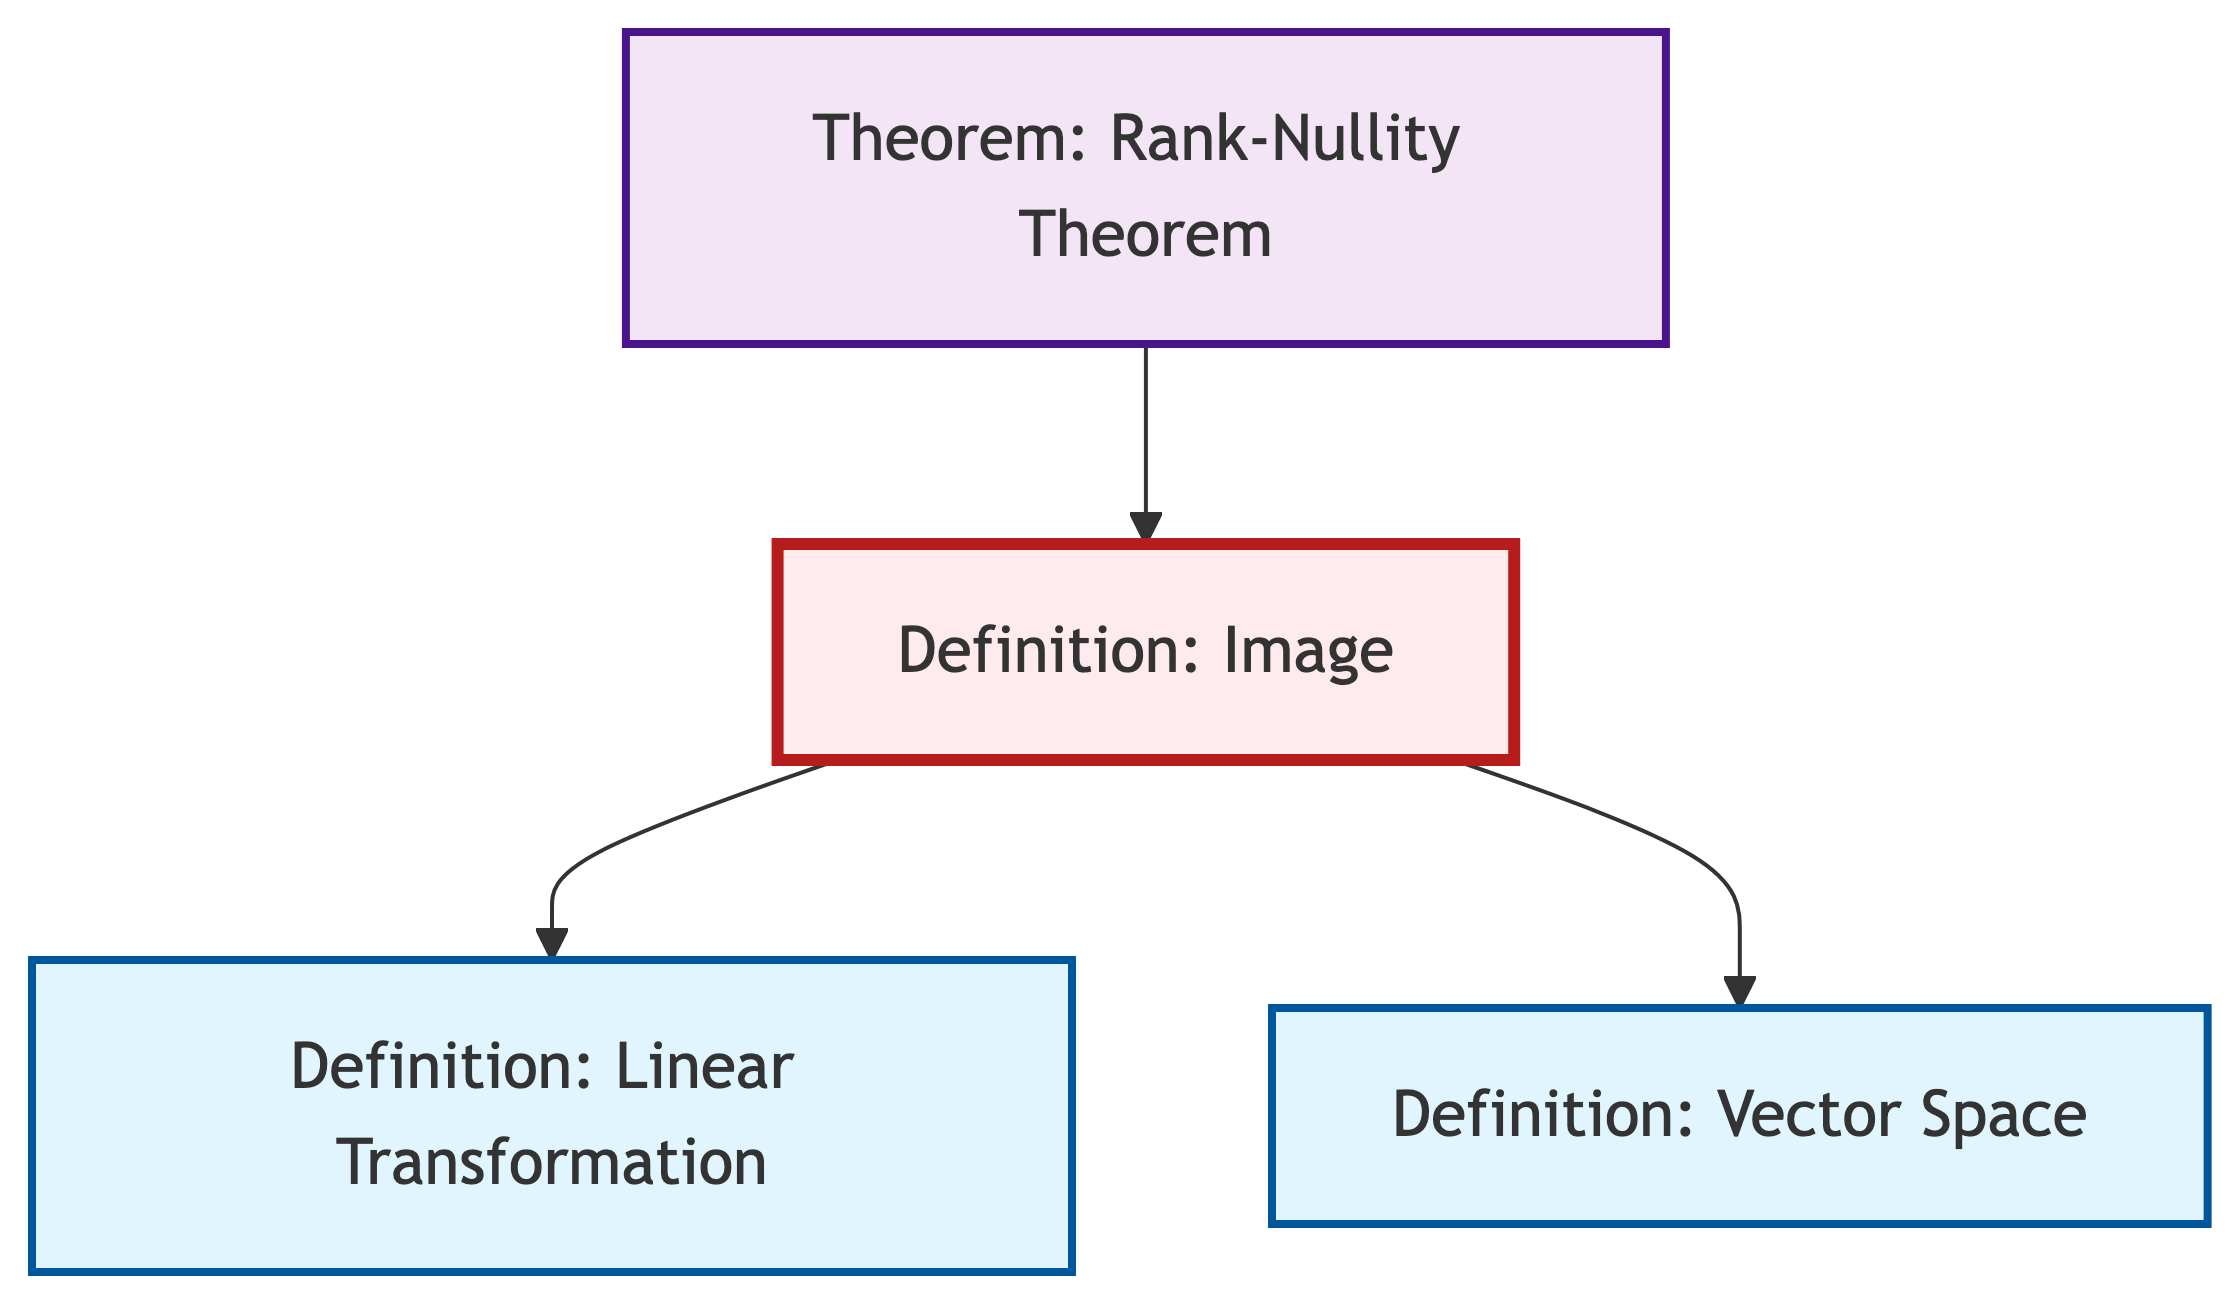
\includegraphics[width=5.83in,height=3.4in]{def-image_files/figure-latex/mermaid-figure-1.png}

Local dependency graph




\end{document}
